% Copyright (c) 2024 RangerOnMars

%*********************************************************************
% RangerOnMars-sauthss: 沈阳航空航天大学本科毕业设计论文模板
% 2024/06/13 v1.0.0
%
% 重要提示:
%   1. 当前overleaf版符合2021研究生学位论文要求,可通过图书馆审核
%   2. 当前版本基于pkuthss v1.9.0
%   3. 请使用UTF-8编码,XeLaTeX方式编译
%   4. 请仔细阅读用户文档
%   5. 修改、使用、发布本文档类请务必遵循LaTeX Project Public License和知识共享4.0
%   6. 如有疑问github/iofu728/pkuthss上提问或联系作者@iofu728
%*********************************************************************

% --------------- 基本信息配置区--------------- 
% 将此处替换为你的中文标题,需要换行处用\\隔开
\newcommand{\getTitle}{{沈阳航空航天大学毕业设计(本科)\\ \LaTeX 模板}}
% 将此处替换为你的英文标题,需要换行处用\\隔开
\newcommand{\getTitleEn}{{SAU Thesis \LaTeX Template for Undergraduate}}
% 将此处替换为你的中文关键词,词和词用;隔开
\newcommand{\getKeywords}{{Latex;沈阳航空航天大学;深度学习}}
% 将此处替换为你的英文关键词,词和词用;隔开
\newcommand{\getKeywordsEn}{{Latex;SAU;Deep Learning}}
% 将此处替换为你的姓名
\newcommand{\getAuthorName}{{李田所}}
% 将此处替换为你的学院
\newcommand{\getInstituteName}{{自动化学院}}
% 将此处替换为你的专业
\newcommand{\getMajorName}{{自动化}}
% 将此处替换为你的班级
\newcommand{\getClassName}{{自动化2001班}}
% 将此处替换为你的学号
\newcommand{\getID}{{20341919810}}
% 将此处替换为你的指导老师
\newcommand{\getMentorName}{{张三}}
% 将此处替换为你的负责教师
\newcommand{\getSupervisiorName}{{王五}}
% 是否在首页放置教师签名png,true为放置
\newcommand{\needMentorsign}{false}% 0 to skip sign, 1 to sign mentor's name.
% 答辩年份
\newcommand{\getYY}{2024}
% 答辩月份
\newcommand{\getMM}{6}
% --------------- 基本信息配置区--------------- 

% -----------沈阳航空航天大学本科生Latex毕设模板------------- 
% 版本:V1.0.0
% Author : RangerOnMars
% Email : guhao0521@gmail.com
% ------------------------------------------------------ 

\documentclass[a4paper,12pt]{article}
\usepackage[fontset=none]{ctex}

\RequirePackage{iftex}
\ifXeTeX\else
    \thss@error{%
      The Overleaf sauthss class requires Xe\TeX{}.\\\\
      You must change your typesetting engine to, e.g.,
      "xelatex" instead of "latex", "lualatex" or "pdflatex".
    }
\fi

% 数学公式和化学方程式
\usepackage{amsmath, amsthm, amssymb, amsfonts}
\usepackage{latexsym,bm}
\usepackage{longtable}
\usepackage{array}
\usepackage[subfigure]{tocloft}
\usepackage[version=4]{mhchem}
\makeatletter
\newcommand{\rmnum}[1]{\romannumeral #1}%小写罗马数字
\newcommand{\Rmnum}[1]{\expandafter\@slowromancap\romannumeral #1@}%大写罗马数字
\makeatother

% 插入PDF文件
\usepackage[final]{pdfpages}

% 引文使用
\usepackage[backend=biber,style=gb7714-2015,gbpub=false]
{biblatex}%align=gb7714-2015
\addbibresource[location=local]{Ref/Collection.bib}

% 插图使用
\usepackage{subfigure, graphicx}
\usepackage{float}
\usepackage{caption}
\usepackage{etoolbox}
\usepackage[hidelinks]{hyperref}
\usepackage{thm-restate}

% 表格使用
\usepackage{bigstrut}
\usepackage{booktabs}
\usepackage{multicol}
\usepackage{multirow}

% LaTeX距离设置:
% mm	毫米	1 mm = 2.845 pt
% pt	点		1 pt = 0.351 mm
% bp	大点	1 bp = 0.353 mm > 1 pt
% dd	迪多	1 dd = 0.376 mm = 1.07 pt
% pc	排卡	1 pc = 4.218 mm = 12 pt
% sp	定标点	65536 sp = 1 pt
% cm	厘米	1 cm= 10 mm= 28.453 pt
% cc	西塞罗	1 cc= 4.513 mm= 12 dd = 12.84 pt
% in	英寸	1 in = 25.4 mm = 72.27 pt
% ex	ex	1 ex = 当前字体尺寸中 x 的高度
% em	em	1 em = 当前字体尺寸中 M 的宽度

% 字体
% \usepackage{fontspec, xunicode, xltxtra}
% \usepackage{xeCJK}
\setmainfont{Times New Roman}
\setsansfont{Droid Sans}
\setmonofont{Courier New}

\setCJKmainfont[Path="Fonts/",AutoFakeBold,ItalicFont=simkai.ttf]{SIMSUN.TTC}
\setCJKsansfont[Path="Fonts/",AutoFakeBold]{SIMHEI.TTF}
\setCJKmonofont[Path="Fonts/",AutoFakeBold]{SIMFANG.TTF}


% 需要的话
\setCJKfamilyfont{zhfs}[Path=Fonts/,AutoFakeBold={2.5}]{SIMFANG.TTF}
\setCJKfamilyfont{zhkai}[Path=Fonts/,AutoFakeBold={2.5}]{SIMKAI.TTF}
\setCJKfamilyfont{zhsong}[Path=Fonts/,AutoFakeBold={2.5}]{SIMSUN.TTC}
\setCJKfamilyfont{zhhei}[Path=Fonts/,AutoFakeBold={2.5}]{SIMHEI.TTF}

\newcommand{\songti}{\CJKfamily{zhsong}}
\newcommand{\heiti}{\CJKfamily{zhhei}}
\newcommand{\fangsong}{\CJKfamily{zhfs}}
\newcommand{\kaishu}{\CJKfamily{zhkai}}

\DeclareCaptionFont{songti}{\songti}
\DeclareCaptionFont{heiti}{\heiti}
\DeclareCaptionFont{fangsong}{\fangsong}
\DeclareCaptionFont{kaishu}{\kaishu}

\usepackage{titlesec}
\usepackage[a4paper,
            left=3.0cm,
            right=3.0cm,
            top=2.6cm,
            bottom=2.6cm,
            headsep=0.7cm,
            footskip=0.7cm]{geometry}
%section等前后间距
\titlespacing*{\section}{0pt}{1ex plus .0ex minus .0ex}{1ex plus .0ex}
\titlespacing*{\subsection}{0pt}{0ex plus .0ex minus .0ex}{0ex plus .0ex}
\numberwithin{equation}{section}
%section等字体设置和字号大小

\usepackage{fancyhdr}
\usepackage{fancybox}
\usepackage{zhnumber}
\usepackage{changepage}
\usepackage{subcaption}
\usepackage{etoolbox}
\usepackage{fancyvrb}  % 用于 verbatim 的高级设置
\usepackage{framed}    % 用于添加边框
% 调整字间距并加框的 verbatim 环境
\RecustomVerbatimEnvironment{Verbatim}{Verbatim}{frame = single, tabsize = 4, fontsize=\footnotesize}

% 防止”孤儿标题“
\makeatletter
% 该函数用于防止标题和内容跨页
\makeatletter
\newcommand{\Needspace}[1]{
    \penalty-100
    \begingroup
    \setlength{\dimen@}{#1}%
    \dimen@ii\pagegoal
    \advance\dimen@ii -\pagetotal
    % \the\baselineskip\the\dimen@:\the\dimen@ii
    \ifdim \dimen@>\dimen@ii
    \ifdim \dimen@ii> \baselineskip
    \vfil
    \fi
    \break
    \fi
    \endgroup
}
% \newcommand{\Needspace}[1]{
%     \penalty-100
%     \begingroup
%     \setlength{\dimen@}{#1}%
%     \dimen@ii\pagegoal
%     \advance\dimen@ii -\pagetotal
%     % \the\baselineskip\the\dimen@:\the\dimen@ii
%     \ifdim \dimen@>\dimen@ii
%         \ifdim \dimen@ii>3\baselineskip
%             \clearpage
%         \else
%             \ifdim \dimen@ii>\baselineskip
%                 \par
%                 \clearpage
%             \else
%                 \break
%             \fi
%         \fi
%     \fi
%     \endgroup
% }
\pretocmd{\Needspace}{\Hy@SaveLastskip}{}{}
\apptocmd{\Needspace}{\Hy@RestoreLastskip}{}{}
\makeatother

\newenvironment{thesisdocument}
{
    % 正文格式
    \zihao{-4}
    \setlength{\baselineskip}{22pt}

    \begin{titlepage}
    %本页为自定义的封面
    \centering
    \quad\\
    \vspace{3.5cm}
	{\heiti\linespread{1.3}\zihao{2}\bfseries\getTitle\\}
 	\vspace{3cm}
	\begin{table}[H]
    	\centering
		  \begin{tabular}{>{\Large}m{3.71cm}>{\arraybackslash\Large}m{6.89cm}}
                {\zihao{-4} 学 \quad 院}&{\zihao{-4} \getInstituteName}\\
                \cline{2-2}\\
                {\zihao{-4} 专 \quad 业}&{\zihao{-4} \getMajorName}\\
                \cline{2-2}\\
                {\zihao{-4} 班 \quad 级}&{\zihao{-4} \getClassName}\\
                \cline{2-2}\\
			{\zihao{-4} 学 \quad 号}&{\zihao{-4} \getID}\\
                \cline{2-2}\\
			{\zihao{-4} 姓 \quad 名}&{\zihao{-4} \getAuthorName}\\
                \cline{2-2}\\
			{\zihao{-4} 指导教师}&{\zihao{-4} \getMentorName}\\
                \cline{2-2}\\
			{\zihao{-4} 负责教师}&{\zihao{-4} \getSupervisiorName}\\
                \cline{2-2}\\
		  \end{tabular}\\
	\end{table}
	\makeatother
        \ifthenelse{\boolean{\needMentorsign}}
        {
            \vspace{1cm}\par
            \hspace{10cm}
            
\includegraphics[height=2cm]{Content/mentor_sign.png}
            \par
        }
        {
            \vspace{3cm}
        }
        {\zihao{-4} \large 沈阳航空航天大学}\\
	{\zihao{-4} \large  \getYY 年 \getMM 月}\\[2cm] % 日期
	\vfill

\end{titlepage}

    % 页眉页脚
    \pagestyle{fancy}
    \fancyhead[L]{}
    \fancyhead[R]{}
    \fancyhead[C]{{\zihao{5}\kaishu\bfseries 沈阳航空航天大学毕业设计(论文)}}
    \fancyfoot[C]{\zihao{-5} \thepage}
    \renewcommand{\headrulewidth}{0.2pt} %页眉横线宽度===========
    
    % 标题格式设置...
    \titleformat{\section}[block]{\vspace*{-5pt}\linespread{1.25}\centering\heiti\zihao{3}\bfseries}{\arabic{section}\vspace{14pt}}{10pt}{}[]
    \titleformat{\subsection}[block]{\vspace{16pt}\zihao{4}\bfseries}{\Needspace{80pt}\linespread{1.73}\arabic{section}.\arabic{subsection}\vspace{16pt}}{10pt}{}[]

    \titleformat{\subsubsection}[block]{\vspace{6pt}\zihao{-4}\bfseries}{\Needspace{80pt}\linespread{1.73}\arabic{section}.\arabic{subsection}.\arabic{subsubsection}\vspace{6pt}}{10pt}{}[]
    
    % 目录格式设置...
    \renewcommand{\cftsecfont}{\zihao{4}\songti} % Section font
    \renewcommand{\cftsecpagefont}{\zihao{4}}
    \setlength{\cftbeforesecskip}{6pt}
    
    \renewcommand{\cftsubsecfont}{\zihao{-4}\songti} % Subsection font
    \renewcommand{\cftsubsecpagefont}{\zihao{-4}}
    \setlength{\cftbeforesubsecskip}{6pt}
    
    \renewcommand{\cftsubsubsecfont}{\zihao{-4}\songti} % Subsubsection font
    \renewcommand{\cftsubsubsecpagefont}{\zihao{-4}}
    \setlength{\cftbeforesubsubsecskip}{6pt}
    
    \renewcommand{\cftdotsep}{1.5}
    \renewcommand{\cftsecleader}{\bfseries\cftdotfill{\cftdotsep}}
    \fancypagestyle{plain}{\pagestyle{fancy}} %解决目录第一页无页眉问题

    % 图片题注格式
    \numberwithin{figure}{section}
    \renewcommand{\thesection}{\arabic{section}}
    \renewcommand{\thefigure}{\thesection.\arabic{figure}}
    \renewcommand{\thesubfigure}{\thesection.\arabic{figure}(\alph{subfigure})}
    \captionsetup[figure]{font={heiti,small,stretch=1.2},labelsep=quad,belowskip=-10pt}
    % 标题题注格式
    \numberwithin{table}{section}
    \captionsetup[table]{font={heiti,small,stretch=1.2},labelsep=quad}
    % \renewcommand\thesubfigure{}
}
{
}

\newenvironment{thesisabstractcn}
{
    \renewcommand{\thepage}{\Roman{page}} % 将页码格式设置为罗马数字
    \phantomsection\addcontentsline{toc}{section}{摘 \quad 要}\tolerance=500 %将摘要放进目录
    {\quad\\\centering \heiti \zihao{3} \bfseries 摘 \quad 要\\[0.9cm]} 
}
{
    \vspace{\baselineskip}
    {\noindent \heiti \zihao{-4} \bfseries 关键词:}
    {\zihao{-4} \getKeywords}\\
    \newpage
}

\newenvironment{thesisabstracten}
{
    \renewcommand{\thepage}{\Roman{page}} % 将页码格式设置为罗马数字
    \phantomsection\addcontentsline{toc}{section}{ABSTRACT}\tolerance=500 %将摘要放进目录
    {\vspace*{-9.5mm}\centering \heiti \zihao{3} \linespread{1.7} \getTitleEn \\[0.6cm]} 
    {\centering \heiti \zihao{3} \bfseries Abstract \\[0.27cm]} 
}
{
    \vspace{\baselineskip}
    {\heiti \zihao{-4} \bfseries Key words:}
    {\noindent \zihao{-4} \getKeywordsEn}
    \newpage
}


\newenvironment{thesisref}
{

    \phantomsection\addcontentsline{toc}{section}{参考文献}\tolerance=500 %将参考文献放进目录
    {\quad\\\centering \heiti \zihao{3} \bfseries 参考文献\\[1cm]}
}
{
    \printbibliography[heading=none]
    \newpage
}

\newenvironment{thesisntfa}
{
    \phantomsection\addcontentsline{toc}{section}{项目非技术因素分析}\tolerance=500 %将非技术分析放进目录
    {\quad\\\centering \heiti \zihao{3} \bfseries 课题方案非技术因素分析\\[1cm]}
}
{
    \newpage
}

\newenvironment{thesisack}
{

    \phantomsection\addcontentsline{toc}{section}{致 \quad 谢}\tolerance=500 %将摘要放进目录
    {\quad\\\centering \heiti \zihao{3} \bfseries 致 \quad 谢\\[1cm]} 
}
{
}



\newenvironment{thesissymboltable}
{
    \renewcommand{\thepage}{\Roman{page}} % 将页码格式设置为罗马数字
    \phantomsection\addcontentsline{toc}{section}{符号表}\tolerance=500 %将摘要放进目录
    {\centering \heiti \zihao{3} \bfseries 符号表\\}
}
{
    \newpage
}

\newenvironment{thesiscontentstable}
{
    \renewcommand{\thepage}{\Roman{page}} % 将页码格式设置为罗马数字
    \phantomsection\addcontentsline{toc}{section}{目\quad 录}\tolerance=500 %将目录放进目录
    \renewcommand*\contentsname{\vspace*{0mm}\heiti \zihao{3} \bfseries 目 \quad 录}
}
{
    \newpage
    \setcounter{page}{1}
}

\newenvironment{thesischapter}
{
    % \newpage
    \renewcommand{\thepage}{\arabic{page}}% 将页码格式设置为罗马数字
}
{
    \newpage
}

%行间距
\usepackage{setspace}

\AtBeginDocument{
    \setlength{\abovedisplayskip}{0.2cm}%公式前后间距,强行在导言区中设置
    \setlength{\belowdisplayskip}{0.2cm}%
    \setlength{\abovedisplayshortskip}{0.2cm}%
    \setlength{\belowdisplayshortskip}{0.2cm}%
    %图片和浮动对象间距
    % \BeforeBeginEnvironment{figure}{\vspace{10pt}}
    \setlength{\floatsep}{0pt plus 0pt minus 0pt}%出现在页面的顶部或底部的浮动对象之间的垂直距离。 缺省为 12pt plus 2pt minus 2pt
    \setlength{\textfloatsep}{15pt plus 0pt minus 0pt}%出现在页面的顶部或底部的浮动对象与文本之间的垂直距离。缺省为 20pt plus 2pt minus 4pt
    \setlength{\intextsep}{10pt plus 0pt minus 0pt}%出现在页面中间的浮动对象(如使用了 h 选项 的浮动对象)与上下方文本之间的垂直距离。 缺省为 12pt plus 2pt minus 2pt
}
% 间距有关变量:
% \baselineskip:行基线间距。
% \lineskip:行间距。
% \baselinestretch:伸展因子。
% \parskip:部分段间距。
% \lineskiplimit:当两行字之间的距离小于\lineskiplimit时,行距自动设为\lineskip。
% 段间距:\lineskip + \parskip
% 行间距:\lineskip = \baselineskip * \baselinestretch

%首行缩进
\usepackage{indentfirst}
\setlength{\parindent}{2pt}

%文本和图片等浮动对象占比
\renewcommand{\floatpagefraction}{.85}%浮动页中浮动对象最大占比
\renewcommand{\textfraction}{.15}%文本页中文本最小占比
\renewcommand{\topfraction}{.65}%页面顶部可以用来放置浮动对象的高度与整个页面高度的最大比例
\renewcommand{\bottomfraction}{.60}

%符号列表间距设置
% \setlength{\leftmargin}{1.2em}%左边界
% \setlength{\parsep}{0ex}%段落间距
% \setlength{\topsep}{1ex}%列表到上下文的垂直距离
% \setlength{\itemsep}{0.5ex}%条目间距
% \setlength{\labelsep}{0.3em}%标号和列表项之间的距离,默认0.5em
% \setlength{\itemindent}{1.1em}%标签缩进量
% \setlength{\listparindent}{0em} %段落缩进量

% 列表格式
\usepackage{enumitem}
% \setlist[enumerate]{listparindent=\parindent}
\setenumerate{label={(\arabic*)},leftmargin=0pt,itemsep=0pt,partopsep=0pt,parsep=\parskip,topsep=5pt,itemindent=4\ccwd}
\setitemize{leftmargin=0pt,itemsep=0pt,partopsep=0pt,parsep=\parskip,topsep=5pt,itemindent=3\ccwd}
\setdescription{leftmargin=0pt,itemsep=0pt,partopsep=0pt,parsep=\parskip,topsep=5pt,itemindent=3\ccwd}
% 代码设置
\usepackage{framed}
\usepackage{listings}
\usepackage{color,xcolor}
\definecolor{DarkBlue}{rgb}{0.05,0,1}
\definecolor{DarkGreen}{rgb}{0.01,0.5,0.04}
\definecolor{DarkPurple}{rgb}{0.67,0.02,0.98}
% 定义一个新的语言
\lstdefinelanguage{MATLAB}
{morekeywords={if,else,end,for,while,break,continue,function}, %定义关键字
sensitive=true, %是否大小写敏感
morecomment=[l]{\%},
morecomment=[l]{\%\%},
morestring=[b]",
morestring=[d]',}
% 代码本体设置
\lstdefinestyle{MATLAB}{
    language=MATLAB,
    basicstyle=\footnotesize\ttfamily,
    backgroundcolor=\color{yellow!10},%背景色淡黄
    frame=shadowbox,
    rulesepcolor=\color{red!20!green!20!blue!20},
    keywordstyle=[1]\color{DarkBlue},  
    keywordstyle=[2]\color{purple},
    keywordstyle=[3]\color{orange}\underbar, 
    stringstyle=\color{DarkPurple},
    commentstyle=\color{DarkGreen},
    numbers=left,
    keepspaces=false,
    numberstyle=\footnotesize,
    % firstnumber=1,
    % stepnumber=1,
}
\lstset{
    basicstyle=\small\ttfamily,%基本样式+小号字体
    frame=trbl,
    %t-top,r-right,b-bottom,l-left
    frameround=tttt,
    %第一个字母表示右上角的拐角,然后顺时针地依次代表各个拐角。f表示方形,t表示弧形
    % showstringspaces=false,
    % identifierstyle=,
    tabsize=4,
    breaklines=true,%自动换行
    % breakautoindent=true,%换行自动缩进
    % breakindent=2em, %缩进距离
    columns=fixed,%固定字间距
    flexiblecolumns,
    xleftmargin=2pt,%左边距
    xrightmargin=0pt,
    aboveskip=5pt,
    belowskip=0pt,
    lineskip=-1pt,%行距增加值
    }

% 算法框图
\usepackage{algorithm}
\usepackage{algpseudocode}
\makeatletter
\def\BState{\State\hskip-\ALG@thistlm}
\makeatother
\floatname{algorithm}{Procedure}
\renewcommand{\algorithmicrequire}{\textbf{Input:}}
\renewcommand{\algorithmicensure}{\textbf{Output:}}

% Tikz流程图
\usepackage{tikz}
\usetikzlibrary{arrows,shapes,chains}
\usetikzlibrary{calc}
% 流程图定义基本形状
\tikzstyle{startstop} = [rectangle, rounded corners, minimum width = 2cm, minimum height=1cm,text centered, draw = black]
\tikzstyle{io} = [trapezium, trapezium left angle=70, trapezium right angle=110, minimum width=2cm, minimum height=1cm, text centered, draw=black]
\tikzstyle{process} = [rectangle, minimum width=3cm, minimum height=1cm, text centered, draw=black]
\tikzstyle{decision} = [diamond, aspect = 3, text centered, draw=black]
% 箭头形式
\tikzstyle{arrow} = [->,>=stealth]

% 页码设置
\pagestyle{empty}

% 水印
\usepackage{eso-pic}
\newcommand\BackgroundPicture{%
  \put(0,0){%
    \parbox[b][\paperheight]{\paperwidth}{%
      \vfill
      \centering%
\begin{tikzpicture}[remember picture,overlay]
\node [rotate=45,scale=6,text opacity=0.3] at (current page.center) {水印样例}; %中括号内是旋转角度,字体大小
\end{tikzpicture}%
      \vfill
    }}}

% 标题样式
% \newcommand\subtitle[1]{{\Large #1}} % 定义副标题
% \makeatletter % change default title style
% \renewcommand*\maketitle{%
%     \begin{center}% 居中标题
%         % \bfseries % 默认粗体
%         {\LARGE\bfseries\@title \par} % LARGE字号,默认粗体
%         \vskip 1em% %%%  标题下面只有1em的缩进或margin
%         {\@author \par}
%         % {\global\let\author\@empty}%
%         {\global\let\date\@empty}%
%         \thispagestyle{empty} %  不设置页面样式
%     \end{center}%
%   \setcounter{footnote}{0}%
% }
\makeatother
\begin{document}
    \begin{thesisdocument}
        % ---------------------------------------------------------------------
        % 论文结构,具体内容在对应tex文件中
        \begin{thesisabstractcn}
    这里是中文摘要内容。\par%意义
    注意事项:概述毕业设计的目的,采用的软硬件设计方案或研究方法、步骤
    等,突出创新点;最终的调试或仿真结果,以及分析得到的研究结论。论文设计
    方案或者采用方法的优点。摘要中不使用公式,不标参考文献。正文小四号,宋
    体,英文和字母采用 Times New Roman 字体。(不少于 600 字)\par
\end{thesisabstractcn}
\begin{thesisabstracten}
    This is English Abstract Content.\par
    The content of English abstract should consist with the content of Chinese abstract.\par
\end{thesisabstracten}
%摘要
        \begin{thesiscontentstable}
    \centering{\thispagestyle{fancy}\tableofcontents}
\end{thesiscontentstable}%目录
        
        \begin{thesischapter}
    \section{绪论}
    本章为sauthss模板的使用示例文档,对本模板的使用时的常见用法和常见问题进行解释和说明。
    \subsection{模板相关}
    本模板是沈阳航空航天大学本科毕设\LaTeX 模板,旨在简化毕业论文写作过程中的格式调整过程。内容与排版部分参考沈阳航空航天大学自动化学院2024年本科毕业设计模板制作并修改。本模板适合有一定编程基础或\LaTeX 写作经验的同学使用。\par
    毕设基本信息在main.tex头部定义,在使用此模板前,请自行按照注释修改相关变量。\par
    \begin{Verbatim}
    % --------------- 基本信息配置区--------------- 
    % 将此处替换为你的中文标题,需要换行处用\\隔开
    \newcommand{\getTitle}{{沈阳航空航天大学毕业设计(本科)\\Latex模板}}
    % 将此处替换为你的英文标题,需要换行处用\\隔开
    \newcommand{\getTitleEn}
    {{SAU Thesis Latex Template for Undergraduate}}
    % 将此处替换为你的中文关键词,词和词用;隔开
    \newcommand{\getKeywords}{{Latex;沈阳航空航天大学;深度学习}}
    % 将此处替换为你的英文关键词,词和词用;隔开
    \newcommand{\getKeywordsEn}{{Latex;SAU;Deep Learning}}
    % 将此处替换为你的姓名
    \newcommand{\getAuthorName}{{李田所}}
    % 将此处替换为你的学院
    \newcommand{\getInstituteName}{{自动化学院}}
    % 将此处替换为你的专业
    \newcommand{\getMajorName}{{自动化}}
    % 将此处替换为你的班级
    \newcommand{\getClassName}{{自动化2001班}}
    % 将此处替换为你的学号
    \newcommand{\getID}{{20341919810}}
    % 将此处替换为你的指导老师
    \newcommand{\getMentorName}{{张三}}
    % 将此处替换为你的负责教师
    \newcommand{\getSupervisiorName}{{王五}}
    % 是否在首页放置教师签名png,true为放置
    \newcommand{\needMentorsign}{false}
    % 答辩年份
    \newcommand{\getYY}{2024}
    % 答辩月份
    \newcommand{\getMM}{6}
    \end{Verbatim}
    \subsection{已知问题}
    本模板当前存在以下主要问题:
    \begin{itemize}
        \item 页面以浮动体(图片、表格)结束时,可能为下一页新的subsection或subsubsection引入多余空行,请调整文本内容与位置尽量避免此情况。\par
        \item 非技术因素分析部分表格布局与Word版表格布局存在一定出入。\par
    \end{itemize}\par
    若您在使用中遇到其他问题,请在github仓库提交Issue或者向此电子邮箱guhao0521@gmail.com发送电子邮件描述您的问题,以便于我们及时解决。您也可以修改代码自行解决问题并向本仓库提交PR,为本项目做出贡献。\par
    \subsection{摘要部分}
    摘要需要在\textbackslash begin\{thesisabstractcn\}和\textbackslash begin\{thesisabstracten\}环境中进行编写。概述毕业设计的目的,采用的软硬件设计方案或研究方法、步骤等,突出创新点;最终的调试或仿真结果,以及分析得到的研究结论。论文设计方案或者采用方法的优点。
    \subsection{目录部分}
    参考本科毕业设计模板制作,分隔点与模板略有出入,不影响实际使用。“目录”二字用三号字、黑体,居中书写,“目”与“录”之间空两格并加粗。一级目录采用四号宋体;二级目录向右缩进 2 字符,采用小四号宋体;三级目录向右缩进 4 字符采用小四号宋体;英文字母和数字都采用 Times New Roman格式;行间距 22 磅(调整\textbackslash cftbeforesecskip得到,实际测量与word行距相同)。
    \subsection{正文部分}
    本模板与word模板相同,采用三级标题形式划分文章。完成内容时请注意标点符号全半角统一,完成一个段落后使用\textbackslash par来结束段落。\par
    下面为标准章节示例代码:\par
    \begin{Verbatim}
    \begin{thesischapter}%开始章节环境
    \section{绪论}%定义章节名称
    % 一些内容
    % ......
    \subsection{研究背景}%二级标题
    % 一些内容
    % ......
    \subsection{国内外研究现状}%二级标题
    \subsubsection{国内研究现状}%三级标题
    % 一些内容
    % ......
    \subsubsection{国外研究现状}%三级标题
    % 一些内容
    % ......
    \end{thesischapter}%结束章节环境
    \end{Verbatim}
    \subsection{图表示例}
    \subsubsection{表格使用示例}
    \begin{table}[h]
        \centering
        \songti\zihao{5}
        \caption{表格示例}
        \begin{tabular}{ccc}
            \toprule
            依赖名称 & 版本需求 & 安装方式 \\
            \midrule
            Ubuntu & 20.04 LTS & 镜像安装 \\
            ROS2 & Foxy & apt安装 \\
            Pytorch & 2.1.0 & pip安装 \\
            CUDA & 12.2 & sh安装 \\
            QT & 5.15 & apt安装 \\
            ifxradarsdk & 3.5.0 & whl安装 \\
            \bottomrule
        \end{tabular}
        \label{tab:sample}
    \end{table}
    毕业设计模板要求表格均使用三线表,表序和表名均位于表格的上方,在Latex中三线表可依赖宏包booktabs实现,使用\textbackslash toprule,
\textbackslash midrule,\textbackslash bottomrule来控制三线。效果如表\ref{tab:sample}所示。 
    \subsubsection{图片使用示例}
     毕业设计模板要求图片题注需位于在图像下方。如图\ref{fig:sample_1}所示。单张图片使用\textbackslash begin\{figure\}环境,若使用Overleaf可直接将图片拖入浏览器以上传图片。注意所有图片均应存储于Figure文件夹下以便于管理。\par
    \begin{figure}[hb]
        \centering
        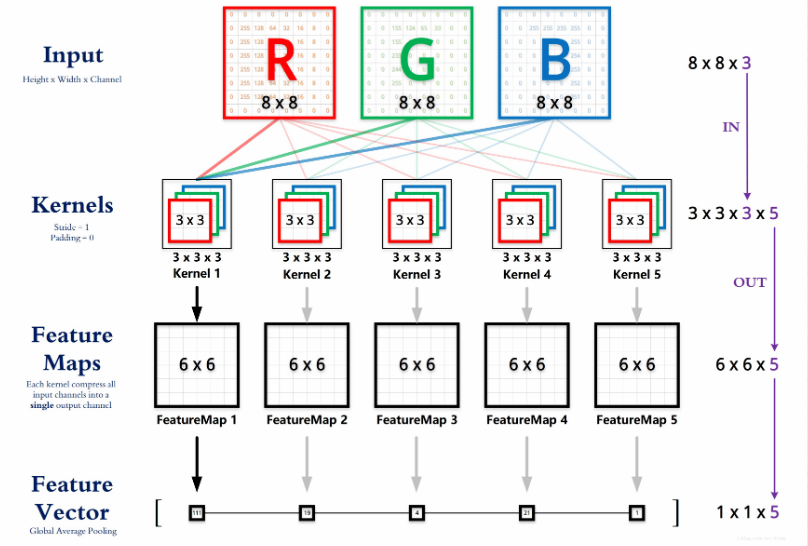
\includegraphics[width=0.4\linewidth]{Figure/sample_1.png}
        \caption{图片样例1}
        \label{fig:sample_1}
    \end{figure}
    当使用多张图片时,可使用subfigure进行插入多张图片。若需引用子图,可以使用\textbackslash subref\{子图label\}进行引用。
    \begin{figure}[h]
        \centering
        \subfigure[常规模块]
        {
            \centering
            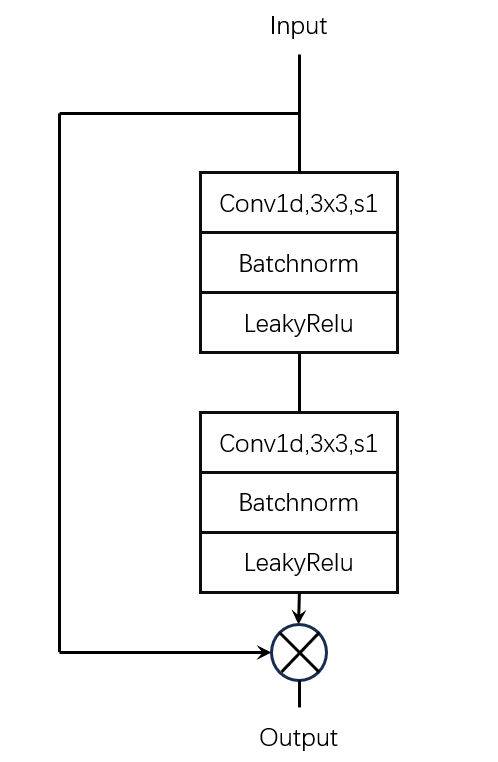
\includegraphics[width=0.44\linewidth]{Figure/resnet1d_flow_a.png}
            \label{fig:resnet1d_flow.a}
        }
        \hfill
        \subfigure[下采样模块]
        {
            \centering
            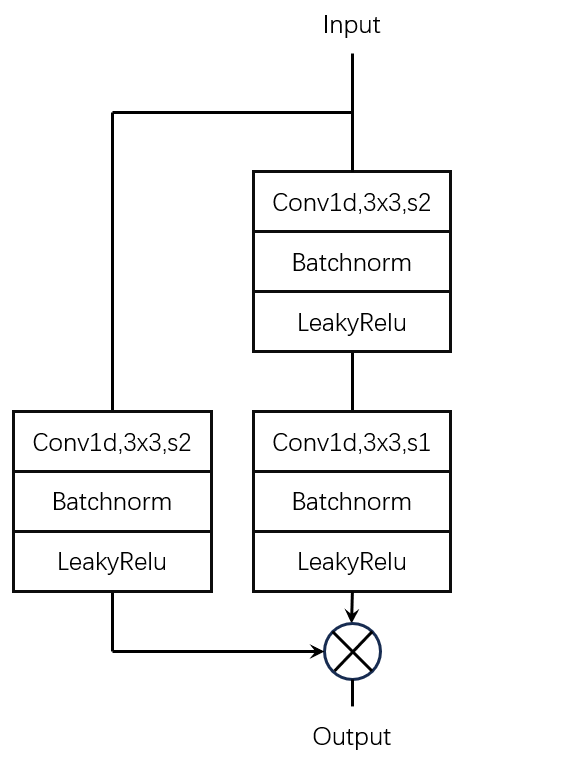
\includegraphics[width=0.52\linewidth]{Figure/resnet1d_flow_b.png}
            \label{fig:resnet1d_flow.b}
        }
        \caption{多张图片示例}
    \end{figure}
    \subsection{公式}
    公式使用\textbackslash begin\{equation\}环境插入,使用通用\LaTeX{}规范即可,如式\ref{eq:mae}。
    \begin{equation}
        MAE = \frac{1}{n} \sum_{i=1}^n |\hat{y}_i - y_i |
        \label{eq:mae}
    \end{equation}\par
    
    \subsection{参考文献}
    参考文献使用GB/T 7714格式进行引用,使用gb7714-2015bibstyle 进行管理,具体引用命令与日常使用类似,\verb|\cite{}|,\verb|\citet{}|,\verb|\citeauthor{}|具体用法见相应文档\cite{hushidong_biblatex-gb7714-2015}。\par
    例如\verb|\cite{feng2018wing}|=\cite{feng2018wing},... 相对于的 bib 文件的书写基本上直接用 Google Scholar 拷贝的 BibTex 即可,部分属性按提示进行微调。\par

    \subsection{版权声明}
    本模板参考Homework in Chinese\cite{overleaf2024homework}模板修改而来。使用文档参考北大本科非官方模板\cite{pku_undergrad_thesis_template}进行编写。\par
    本示例文档和模板遵循 LATEX Project Public License 和 Attribution 4.0 International (CC BY 4.0) 开源协议。
\end{thesischapter}%具体章节,下同
        \begin{thesischapter}
    \section{第二章}
    第二章内容...
\end{thesischapter}
        \begin{thesischapter}
    \section{第三章}
    第三章内容...\par
        
\end{thesischapter}
        \begin{thesischapter}
    \section{第四章}
    第四章内容...\par
\end{thesischapter}
        \begin{thesischapter}
    \section{第五章}
    第五章内容...\par
\end{thesischapter}
        \begin{thesischapter}
    \section{第六章}
    第六章内容...\par
\end{thesischapter}
        \begin{thesischapter}
    \section{第七章}
    第七章内容...\par
\end{thesischapter}
        \begin{thesisntfa}
    \flushleft
    \renewcommand\arraystretch{1.8}
    \begin{longtable}{p{1.78cm}|p{1.27cm}|p{1.27cm}|p{8.46cm}}
        \hline
        \multirow{2}{*}{\shortstack{非技术\\因素}} & \multicolumn{2}{l|}{\shortstack{是否为项目\\主要影响因\\素(√)}} & \multirow{2}{*}{\centering\shortstack{简述非技术因素对项目的影响\\及项目设计过程中对应采取的措施}} \\
        \cline{2-3}
        \rule{0pt}{1cm} & 是 & 否 & \\
        \hline
        \endhead
        成本 & √ &  & 设计系统时考虑到日后NPU部署移除上位机以减小成本的需求,对模型尽可能的进行了轻量化。 \\
        \hline
        % 表格内容开始
        经济性 &  & √ &  \\
        \hline
        社会 &  & √ & \\
        \hline
        健康 & √ &  & 该设备的推出可以辅助特殊人群监控健康状态,并让患者及时进行自我调整。有助于提高国民健康水平。 \\
        \hline
        安全 &  & √ & \\
        \hline
        法律 & √ &  & 数据采集时考虑到生理数据的敏感属性,受试者在接受数据采集之前均已签署知情同意书。\\
        \hline
        文化 &  & √ & \\
        \hline
        环境 &  & √ & \\
        \hline
        其他 &  & √ & \\
        \hline
    \end{longtable}
\end{thesisntfa}%非技术因素分析
        \begin{thesisref}
\end{thesisref}%引用
        \begin{thesisack}
    这里是一些致谢内容...
    \newpage
\end{thesisack}%致谢
    \end{thesisdocument}
\end{document}